\documentclass{article}

\usepackage[utf8]{inputenc}


\usepackage{geometry}
\usepackage{xcolor}
%\usepackage{graphix}
\usepackage{tikz}
\usepackage{mathtools}
\usepackage{pgfplots}
\usepackage{algorithm}
\usepackage[noend]{algpseudocode}
\usepackage{amsmath}
\usepackage{amsfonts}
\usepackage{amssymb}
\usepackage[backend=biber]{biblatex}


\addbibresource{citations.bib}


\renewcommand{\algorithmicrequire}{\textbf{Input:}}
\renewcommand{\algorithmicensure}{\textbf{Output:}}

\definecolor{gradient1}{HTML}{833ab4}
\definecolor{gradient2}{HTML}{fd1d1d}
\definecolor{gradient3}{HTML}{fc8a3b}
\definecolor{gradient4}{HTML}{fcb045}


\geometry{top=2cm, bottom=2cm, left=2cm, right=2cm}

\title{Final Project\\ INF236: Parallel Programming\\ Parallel Matrix Multiplication}

\author{Kate\v{r}ina \v{C}\'{i}\v{z}kov\'{a}, Luca Klingenberg}


\begin{document}

\maketitle

\section{Introduction}

\section{Algorithms}
In this section all the implemented algorithms are explained in further detail.

\subsection{Matrix Multiplication}

\begin{algorithm}[H] 
\caption{Matrix Multiplication}
\label{alg:matmul}
\begin{algorithmic}[1]
\Require{$\mathbf{A}, \mathbf{B}$} %Input
\Ensure{$\mathbf{C}$ (the resulting matrix)} %Output
\Statex
\Function{matmul}{$\mathbf{A}, \mathbf{B}$}
	\For{$i=0, \ldots, n-1$}
		\For {$j=0, \ldots, n-1$}
			\State {$c[i][j] = 0$}
		\EndFor
		\For{$k=0, \ldots, n-1$}
			\For{$j=0, \ldots, n-1$}
				\State {$c[i][j] += a[i][k] * b[k][j]$}
			\EndFor
		\EndFor
	\EndFor
	\State \Return {$\mathbf{C}$}
\EndFunction
\end{algorithmic}
\end{algorithm}

\subsection{Strassen Algorithm}

\begin{algorithm}[H] 
\caption{Strassen Matrix Multiplication}
\label{alg:strassen}
\begin{algorithmic}[1]
\Require{$\mathbf{A}, \mathbf{B}$} %Input
\Ensure{$\mathbf{C}$ (the resulting matrix)} %Output
\Statex
\Function{strassen}{$\mathbf{A}, \mathbf{B}, n$}
	\If {n == cutoff}
		\State \Return {$\mathbf{A} * \mathbf{B}$}
	\EndIf
	\State {$\mathbf{P}_1 = strassen(\mathbf{A}_{00} + \mathbf{A}_{11},  \mathbf{B}_{00} + \mathbf{B}_{11}, \frac{n}{2})$}
	\State {$\mathbf{P}_2 = strassen(\mathbf{A}_{10} + \mathbf{A}_{11},  \mathbf{B}_{00}, \frac{n}{2})$}
	\State {$\mathbf{P}_3 = strassen(\mathbf{A}_{00},  \mathbf{B}_{01} - \mathbf{B}_{11}, \frac{n}{2})$}
	\State {$\mathbf{P}_4 = strassen(\mathbf{A}_{11},  \mathbf{B}_{10} - \mathbf{B}_{00}, \frac{n}{2})$}
	\State {$\mathbf{P}_5 = strassen(\mathbf{A}_{00} + \mathbf{A}_{01},  \mathbf{B}_{11}, \frac{n}{2})$}
	\State {$\mathbf{P}_6 = strassen(\mathbf{A}_{10} - \mathbf{A}_{00},  \mathbf{B}_{00} + \mathbf{B}_{01}, \frac{n}{2})$}
	\State {$\mathbf{P}_7 = strassen(\mathbf{A}_{01} - \mathbf{A}_{11},  \mathbf{B}_{10} + \mathbf{B}_{11}, \frac{n}{2})$}
	\State {$\mathbf{C}_{00} = \mathbf{P}_1 + \mathbf{P}_4 - \mathbf{P}_5 + \mathbf{P}_7$}
	\State {$\mathbf{C}_{01} = \mathbf{P}_3 + \mathbf{P}_5$}
	\State {$\mathbf{C}_{10} = \mathbf{P}_2 + \mathbf{P}_4$}
	\State {$\mathbf{C}_{11} = \mathbf{P}_1 - \mathbf{P}_2 + \mathbf{P}_3 + \mathbf{P}_6$}
	 	
	\State \Return {$\mathbf{C}$}
\EndFunction
\end{algorithmic}
\end{algorithm}

\subsection{Parallel Matrix Multiplication}

\subsection{Parallel Strassen Algorithm}

\section{Experiments}
	
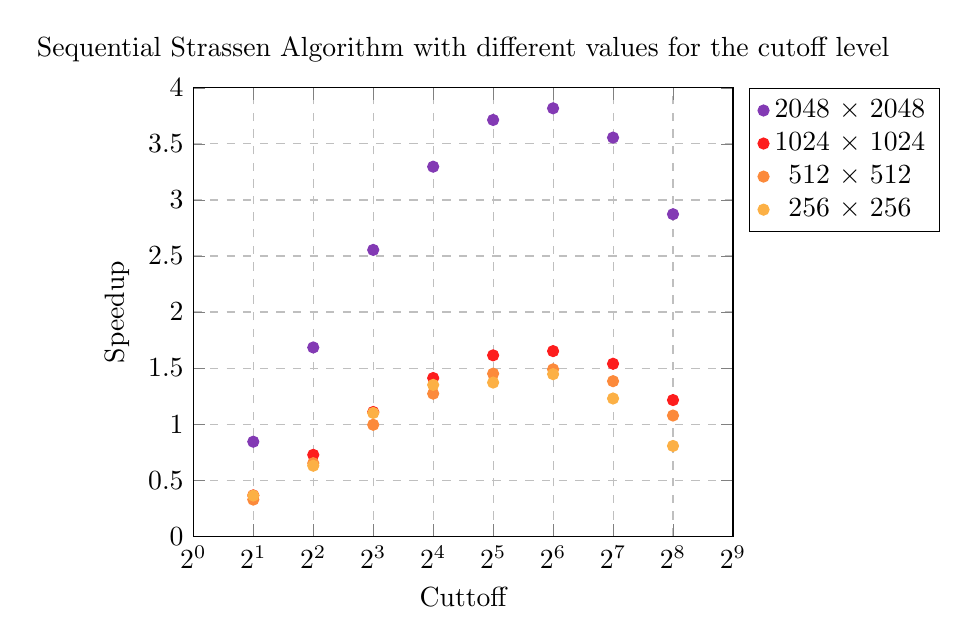
\begin{tikzpicture}
\begin{axis}[
    title={Sequential Strassen Algorithm with different values for the cutoff level},
    xlabel={Cuttoff},
    ylabel={Speedup},
    xmin=1, xmax=512,
    ymin=0, ymax=4,
    xtick={0,1,2,4,8,16,32,64,128,256,512},
    ytick={0, 0.5, 1, 1.5, 2, 2.5, 3, 3.5, 4},
	xmode=log,
    log basis x={2},
    legend pos=outer north east,
    xmajorgrids=true,
    ymajorgrids=true,
    grid style=dashed,
]

 \addplot[
    color=gradient1,
    mark=*,
    only marks,
    ]
    coordinates {
    % running time of normal sequential: 22.729855
     (2, 0.8429769135)(4, 1.6839890956)(8, 2.5542670016)(16, 3.2968112104)(32, 3.7138089218)(64, 3.8177959134)(128, 3.556450524)(256, 2.8727691346)
    };

 \addplot[
    color=gradient2,
    mark=*,
    only marks,
    ]
    coordinates {
    % running time of normal sequential: 1.397876
     (2, 0.3643141647)(4, 0.7259570318)(8, 1.1082371204)(16, 1.4111962817)(32, 1.613661235)(64, 1.6513519133)(128, 1.5385655071)(256, 1.2147025062)
    };

\addplot[
    color=gradient3,
    mark=*,
    only marks,
    ]
    coordinates {
    % running time of normal sequential: 0.177942
     (2, 0.3265631968)(4, 0.6516255667)(8, 0.9941393701)(16, 1.2717773521)(32, 1.4503146089)(64, 1.4886806659)(128, 1.3831910825)(256, 1.0765442556)
    };
    
    \addplot[
    color=gradient4,
    mark=*,
    only marks,
    ]
    coordinates {
    % running time of normal sequential: 0.032513
     (2, 0.3625648174)(4, 0.6287808463)(8, 1.0997496956)(16, 1.350095507)(32, 1.3708154145)(64, 1.4456647399)(128, 1.2285623673)(256, 0.8052157115)
    };
    \legend{2048 $\times$ 2048, 1024 $\times$ 1024, 512 $\times$ 512, 256 $\times$ 256}
    
    
    
\end{axis}
\end{tikzpicture}

\section{Conclusion}

\printbibliography

\end{document}